\chapter{Мотивация}

https://www.viva64.com/ru/b/0438/



Приведем примеры катастроф, приведших к человеческим жертвам, большим экономическим потерям,
по причине наличия ошибок или недочетов в программно-аппаратных комплексах.
\begin{itemize}
    \item Ariane 5 \cite{journal:open_system:1998_adjaev}\footnote{\url{http://www.osp.ru/os/1998/06/179592}}
    про наследуемую систему навигации,
    у которой входные параметры вышли за пределы доппустимого значения,
    выработолась исключительная ситуация из-за чего, система навигация переключилась на резервную систему,
    которая также получила недопустимые входные значения, повторив отбраковку прибора.
    Эти исключительные ситуации перехватила БЦВЭМ, которая так же была автоматикой 
    распознана аварийной и выключена.
    %
    \item Therac-25 \cite{journal:computer:1993:therac25} рисунки \ref{fig:therac25, fig:therac25_console} переоблучение пациентов (несколько литальных исходов) в следствии некоректной синхроницации,
    между системой ввода параметров (момент нахождения коретки) и проверка введенных параметров,
    на допустимох и взаимную совместимость.
    %
    \item Блэкоут в 2003 году\footnote{\url{https://m.habr.com/ru/company/mailru/blog/370153/}}.
    %
    \item Запуск балистических ракет в 1983 году (там же).
    %
    \item Смена часового пояса у истребителей F-22. 
\end{itemize}

\begin{figure}
    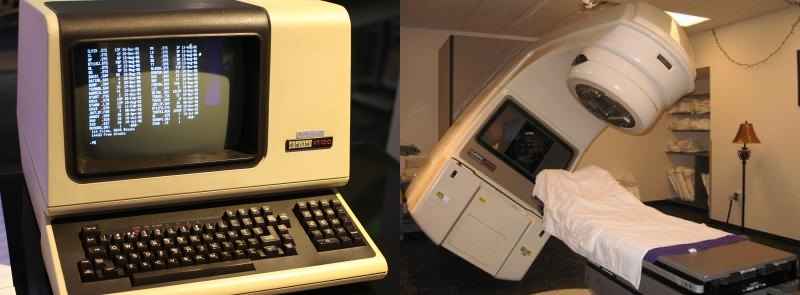
\includegraphics{therac25-console}
    \caption{Therac 25}\label{fig:therac25}
    %
    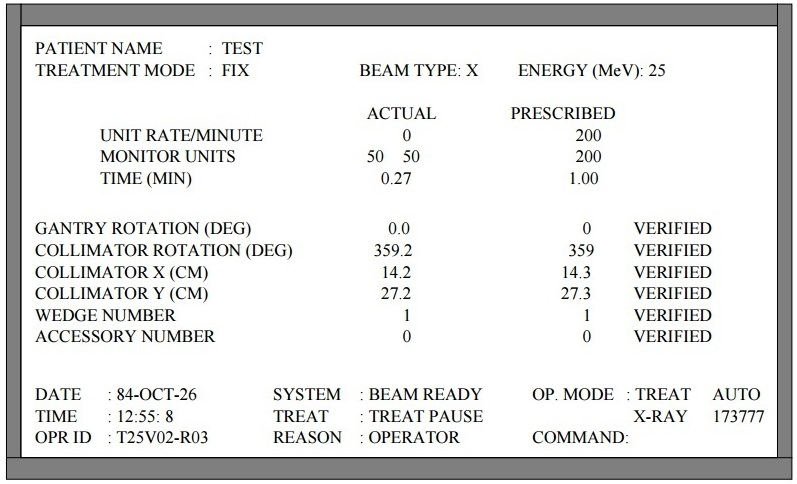
\includegraphics{therac25-screenshot}
    \caption{Консоль Therac 25}\label{fig:therac25_console}
\end{figure}

Нужно ещё примеров \ldots

конечно ни одно программное неможет бытьпроверенно полностью (ссылка на авторитета).

\chapter{Протокол Modbus}\label{ch:ch1}

\section{Описание протокола}

\section{Обзор существующих решений}\label{sec:ch1/sec1}
\subsection{QSlave}

В свободном продукте\footnote{\url{https://github.com/maisvendoo/qslave}}, распространяемом по лиценции GPL используется
реализация имитатора множества конечных устройств, которые объеденены в одну сеть.
Этот программный продукт не подходит так как связь реализована по протоколу
Modbus/RTU, так как в конечном продукте необходима реализация через Modbus/TCP~IP.

\subsection{mEmulator}
Другой продукт\footnote{\url{http://ardsoft.ru/mEmulator.html}} требует исследования.


\subsection{Еще продукты}


\section{Выводы по существующим решениям}

Так как ни одно из решений не соответствует требованиям, придется реализовать свой
имитатор, архитектрура которого описана далее в главе \ref{sec:ch2}.